%!TEX root = tfg.tex
\chapter{Entorno de simulación y desarrollo}

\begin{quotation}[Presidente de Estados Unidos]{Abraham Lincoln (1809--1865)}
Dame seis horas para cortar un árbol y pasaré las primeras cuatro afilando el hacha.
\end{quotation}

\begin{abstract}
Este capítulo describe el entorno concreto sobre el que se ha desarrollado el proyecto: el simulador utilizado, las características del hardware de desarrollo y las herramientas software que han facilitado la implementación y depuración del sistema.
\end{abstract}

\section{Entorno de simulación}

\begin{figure}[H]
    \centering
    \begin{minipage}{0.28\textwidth}
        \centering
        
\includegraphics[width=\textwidth]{figures/logos/ubuntu_2204_logo}
        \caption{Ubuntu 22.04 LTS.}
        \label{fig:logo_ubuntu}
    \end{minipage}
    \hfill
    \begin{minipage}{0.28\textwidth}
        \centering
        
\includegraphics[width=\textwidth]{figures/posters/ros2_humble_poster}
        \caption{ROS2 Humble Hawksbill.}
        \label{fig:logo_humble}
    \end{minipage}
    \hfill
    \begin{minipage}{0.28\textwidth}
        \centering
        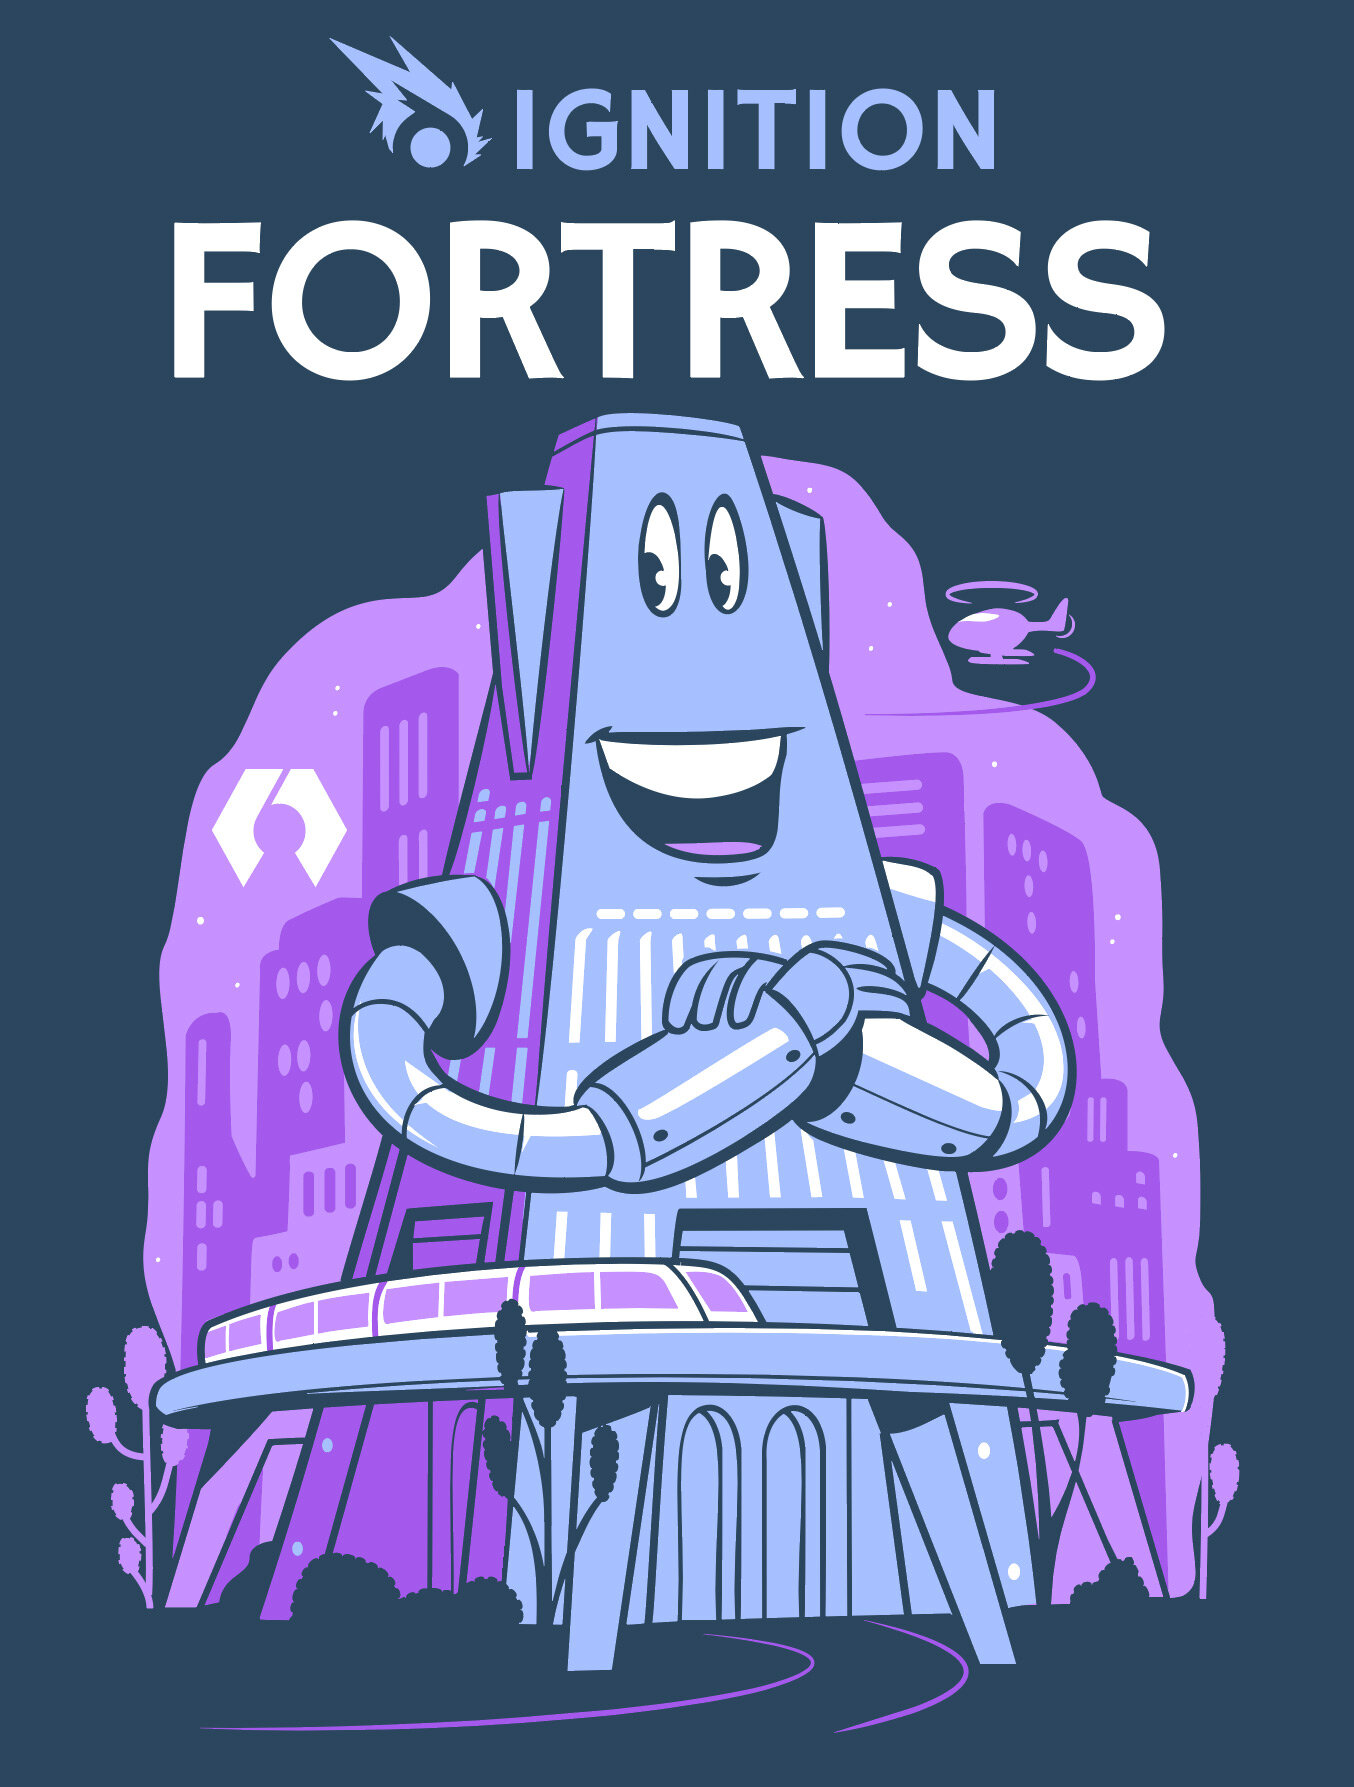
\includegraphics[width=\textwidth]{figures/posters/ignition_fortress_poster}
        \caption{Ignition Gazebo Fortress.}
        \label{fig:logo_fortress}
    \end{minipage}
\end{figure}

El entorno de simulación empleado es \textbf{Ignition Gazebo Fortress}, lanzado sobre \textbf{Ubuntu 22.04 LTS} con \textbf{ROS2 Humble}. Para las pruebas de navegación se ha utilizado el mundo \texttt{warehouse.sdf}, un almacén industrial incluido en los paquetes oficiales del TurtleBot4 que dispone de estanterías, pasillos y obstáculos distribuidos en un espacio de aproximadamente $30 \times 20$ metros. Este entorno presenta suficiente complejidad geométrica para evaluar el comportamiento de los algoritmos de planificación ante obstáculos y trayectorias con diferentes grados de dificultad.

Para la localización se ha utilizado el mapa del almacén (\texttt{warehouse.pgm} y \texttt{warehouse.yaml}) incluido en el paquete \texttt{turtlebot4\_navigation}, que proporciona una representación 2D del entorno a 3\,cm por celda. Este mapa se carga al arrancar el sistema y se utiliza como referencia para AMCL y el planificador global de Nav2.

La figura~\ref{fig:lidar_global} muestra una captura del entorno de simulación visualizado en RViz2, donde se puede apreciar el mapa del almacén junto con las lecturas del LiDAR (en rojo) que el robot percibe en tiempo real desde su posición.

\begin{figure}[H]
    \centering
    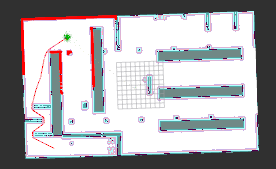
\includegraphics[width=0.75\textwidth]{figures/screenshots/puntos-lidar-global_menos-resolucion-mejor-vision}
    \caption{Vista global del almacén en RViz2 con las lecturas del LiDAR (rojo) y la trayectoria planificada.}
    \label{fig:lidar_global}
\end{figure}

Una limitación relevante del entorno de simulación es el rendimiento. En el hardware de desarrollo principal (un portátil con procesador Intel Core i5 y gráficos integrados) la simulación corre a aproximadamente el 20\% de la velocidad real, lo que dificulta la navegación autónoma y hace que los comportamientos de temporización (timeouts, frecuencias de publicación) requieran ajustes respecto a sus valores nominales. Esta limitación se ha mitigado parcialmente utilizando un PC de alto rendimiento del departamento para las pruebas con el nodo de métricas dinámico, como se describe en la siguiente sección.

\section{Hardware de desarrollo}

El desarrollo se ha realizado sobre dos máquinas con diferentes características:

\textbf{Portátil de desarrollo (principal):} Intel Core i5, gráficos integrados, Ubuntu 22.04 LTS con ROS2 Humble instalado de forma nativa. Se ha utilizado para el desarrollo de los nodos C++, la configuración de Nav2 y las pruebas con el nodo de métricas estático. La simulación corre al $\approx$20\% de la velocidad real en este hardware.

\textbf{PC del departamento (experimentos dinámicos):} Intel Core i7-14700F (20 núcleos), GPU NVIDIA GeForce RTX 3050 6\,GB, Ubuntu 24.04 LTS. Dado que Ubuntu 24.04 no es la plataforma oficial de ROS2 Humble, se ha empleado \textbf{Docker}\cite{docker} con la imagen oficial \texttt{osrf/ros:humble-desktop-full}, basada en Ubuntu 22.04, para garantizar la compatibilidad. El acceso a la GPU desde el contenedor se habilita mediante \texttt{nvidia-container-toolkit}, lo que permite que Ignition Gazebo use aceleración hardware y la simulación corra al 85--100\% de la velocidad real. Este entorno se ha utilizado para las pruebas con el nodo de métricas dinámico, que requiere que el robot navegue correctamente hasta el destino.

Para garantizar la reproducibilidad del entorno Docker en cualquier máquina, se incluye en el repositorio un \texttt{Dockerfile} que automatiza la instalación de ROS2 Humble y los paquetes necesarios del TurtleBot4 a partir de la imagen base.

\section{Herramientas de desarrollo}

\subsection{RViz2}

\begin{figure}[H]
    \centering
    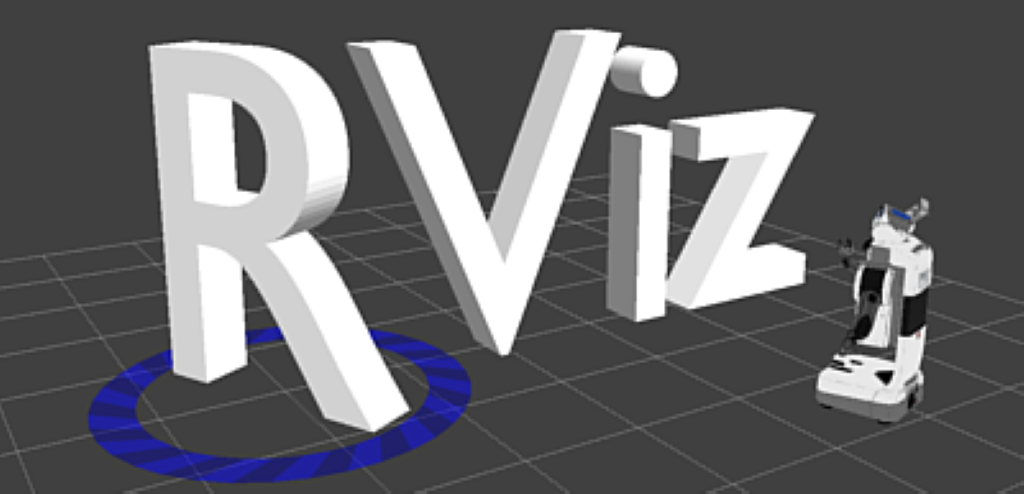
\includegraphics[width=0.40\textwidth]{figures/logos/rviz2_logo}
    \caption{Logo de RViz2.}
    \label{fig:logo_rviz2}
\end{figure}

\textbf{RViz2} es la herramienta de visualización estándar de ROS2. Se ha utilizado a lo largo de todo el proyecto para visualizar el estado del robot, el mapa, el costmap, las trayectorias planificadas y los datos del LiDAR en tiempo real. También proporciona herramientas interactivas como el botón \textit{2D Pose Estimate} para establecer la pose inicial de AMCL y el botón \textit{Nav2 Goal} para enviar objetivos de navegación de forma manual.

La figura~\ref{fig:rviz_costmap} muestra un ejemplo de la información visualizada en RViz2 durante la navegación: el costmap con el inflado de obstáculos (en tonos magenta y cian), el robot en su posición actual y la trayectoria planificada (en rosa). Es posible apreciar cómo el planificador genera un camino que rodea los obstáculos respetando la zona de inflado.

\begin{figure}[H]
    \centering
    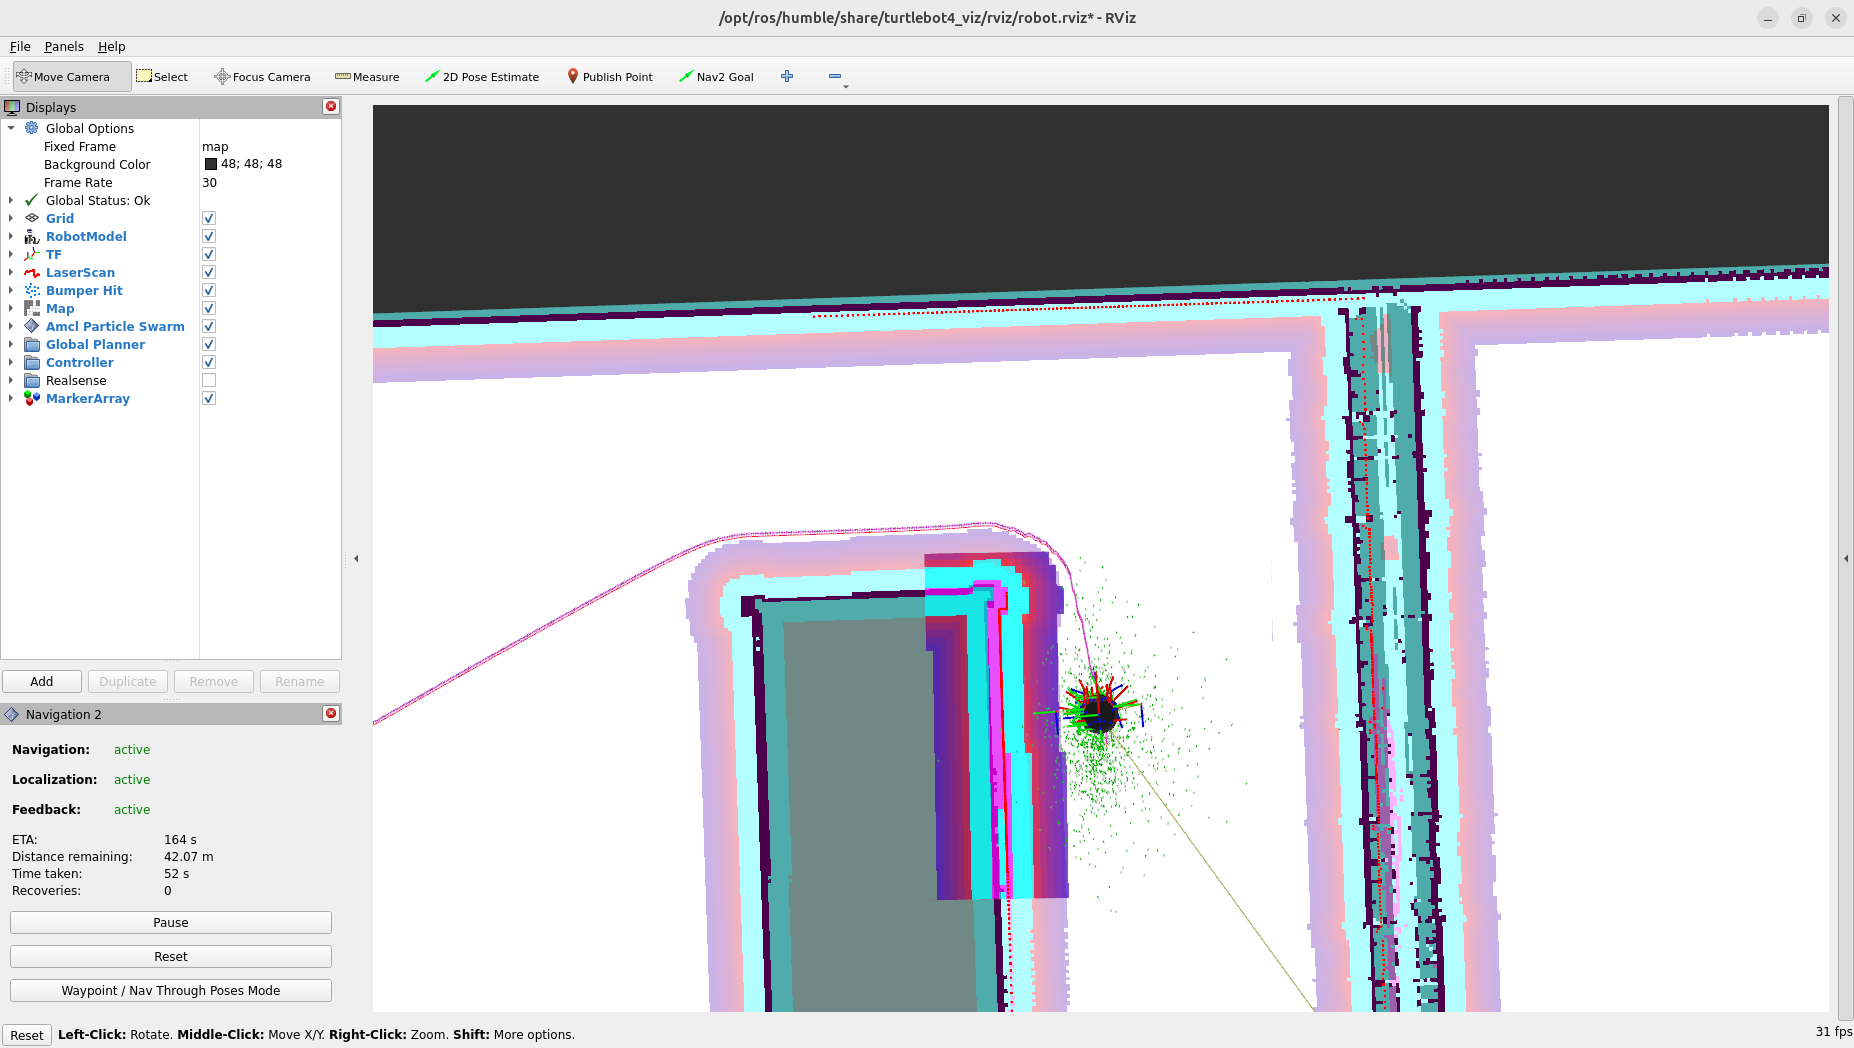
\includegraphics[width=0.75\textwidth]{figures/screenshots/lidar-en-borde-y-giro-estanteria}
    \caption{RViz2 mostrando el costmap, el robot y la trayectoria planificada al rodear una estantería.}
    \label{fig:rviz_costmap}
\end{figure}

\subsection{Herramientas de diagnóstico de ROS2}

Durante el desarrollo se han utilizado diversas herramientas de línea de comandos de ROS2 para depuración y diagnóstico:

\begin{itemize}
    \item \texttt{ros2 topic echo/list/hz/info}: para inspeccionar los mensajes publicados en los topics y verificar frecuencias de publicación.
    \item \texttt{ros2 node info}: para ver las suscripciones, publicaciones y servicios de un nodo.
    \item \texttt{ros2 param get/set}: para leer y modificar parámetros de nodos en tiempo de ejecución.
    \item \texttt{ros2 action send\_goal}: para enviar goals a action servers como el undock o el spin del Create3.
    \item \texttt{tf2\_tools view\_frames}: para visualizar el árbol de transformadas TF del sistema, herramienta fundamental para diagnosticar problemas de localización.
\end{itemize}

\subsection{Visual Studio Code}

\begin{figure}[H]
    \centering
    
\includegraphics[width=0.40\textwidth]{figures/logos/vscode_logo}
    \caption{Logo de Visual Studio Code.}
    \label{fig:logo_vscode}
\end{figure}

El editor principal de desarrollo ha sido \textbf{Visual Studio Code}\cite{vscode}, con las siguientes extensiones que mejoran significativamente la experiencia de desarrollo en el ecosistema ROS2/C++:

\begin{itemize}
    \item \textbf{Robotics Developer Environment (Ranch Hand Robotics):} suite de extensiones específicamente diseñada para el desarrollo con ROS2. Proporciona autocompletado de tipos de mensajes, integración con el sistema de build de ROS2 y herramientas de depuración adaptadas al ecosistema. Se optó por esta extensión en lugar de la extensión oficial \textit{ROS} de Microsoft, que ha sido marcada como \textit{deprecated} y ya no recibe mantenimiento activo.
    \item \textbf{CMake Tools:} soporte para proyectos CMake, que es el sistema de construcción utilizado por los paquetes ROS2 (\texttt{ament\_cmake}).
    \item \textbf{CMake:} resaltado de sintaxis e IntelliSense para archivos \texttt{CMakeLists.txt}.
    \item \textbf{C/C++ (Microsoft):} IntelliSense, depuración y navegación de código para C++, incluyendo soporte para las cabeceras de ROS2.
    \item \textbf{LaTeX Workshop:} edición y compilación de la memoria del TFG directamente desde VSCode.
\end{itemize}

\subsection{Python y análisis de datos}

Para el análisis de los resultados experimentales se ha desarrollado un proyecto Python independiente (\texttt{ros2/Analysis/}) con un entorno virtual aislado. Las librerías principales utilizadas son \textbf{pandas} para la manipulación de los CSV de métricas, \textbf{matplotlib} y \textbf{seaborn} para la generación de gráficas comparativas, y \textbf{numpy} para los cálculos numéricos.
